\begin{tikzpicture}[x=1cm,y=1cm,font=\small]
  \fill[orange!22] (3.5,0)--(0,3)--(7.5,3)--cycle;
  \fill[blue!9] (3.5,0)--(7.5,3)--(10,3)--cycle;
  \foreach \position in {2.5,5,7.5}
    \draw[gray!70,dashed] (3.5,0)--(\position,3);
  \draw[thick] (3.5,0)--(0,3)--(10,3)--cycle;
  \fill (3.5,0) circle (2.2pt) node[below] {$0$};
  \fill (0,3) circle (1.8pt) node[left] {$u$};
  \fill (10,3) circle (1.8pt) node[right] {$v$};
  \foreach \position/\width in {1.25/\ell,3.75/\cdots,6.25/\ell,8.75/w_0}
    \node[above] at (\position,3.05) {$\width$};
  \draw[thin] (0,3.55)--(0,3.95);
  \draw[thin] (10,3.55)--(10,3.95);
  \draw[<->] (0,3.8)--(10,3.8) node[midway,above] {$E:\quad w=m\ell+w_0$};
  \node[fill=orange!22,inner sep=2pt] at (3.5,2.45) {$m$ primitive $T$-triangles};
  \draw[gray!70,dotted] (3.5,0)--(10.9,0);
  \draw[gray!70,dotted] (10,3)--(10.9,3);
  \draw[<->] (10.75,0)--(10.75,3) node[midway,right] {$\ell$};
  \node[text=orange!65!black] at (2.7,-0.75) {$T$-part: $m\binom{\ell}{2}$};
  \node[text=blue!70!black] at (8.3,-0.75) {residue: $\dfrac{w_0(\ell-1)}2$};
  \node at (5.2,-1.65)
    {$\displaystyle\frac{w(\ell-1)}2=m\binom{\ell}{2}+\frac{w_0(\ell-1)}2$};
\end{tikzpicture}